 \documentclass[11pt,a4paper]{article}
\usepackage[utf8]{inputenc}
\usepackage[finnish]{babel}
\usepackage[T1]{fontenc}
\usepackage{amsmath}
\usepackage{amsfonts}
\usepackage{amssymb}
\usepackage{amsthm}
\pagestyle{plain}
\usepackage{graphicx}
\title{Mikroskaalapelkistys - 
\\Kaupallisen ketonin stereokemia}
\author{Delun Li\\014631300\\Orgaanisen kemian työt\\Työ 2}
\date{11.10.2018}


\begin{document}

\maketitle

\pagebreak

\section{Johdanto}

\noindent Työssä selvitettiin kaupallisen ketonin (2,6-dimetyylisykloheksanoni) stereokemiaa, sillä kaupallisen ketonin isomeerien suhde riippuu pelkistetyistä tuotteiden, 2,6-dimetyyliheksanoli, isomerioista.$^1$ Suhdetta tarkastettiin GC:lla (kaasukromatokrafia). 


\vspace{0.3cm}

\noindent \textbf{Reaktioyhtälö:}

\vspace{0.3cm}

\hspace{0.7cm}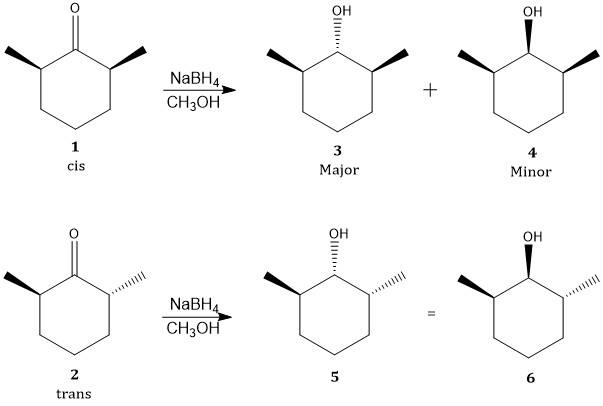
\includegraphics[height = 7cm, width = 10cm]{mikroskaalayht.jpg}

\noindent Kaupallisessa ketonissa löytyy \textit{cis}- (\textbf{1}) ja \textit{trans}-isomerioita (\textbf{2}). Yllä olevassa reaktioyhtälössä on esitetty mitä tuotteita syntyy pelkistettäessä eri ketoni-isomerioita. 

Pelkistettäessä isomeriaa \textbf{1} NaBH$_4$:llä, saadaan tuotteeksi \textit{trans,trans}-2,6-dimetyyli\- sykloheksanoli, \textbf{3}, ja \textit{cis,cis}-2,6-dimetyyliheksanoli, \textbf{4}. Toisaalta, kun pelkistetään \textbf{2} saadaan tuotteeksi enantiomeerit \textit{cis,trans}-2,6-dimet\- yylisykloheksanolia, \textbf{5} ja \textbf{6}.


\vspace{1cm}

\noindent \textbf{Reaktiomekanismi:}

\vspace{0.3cm}

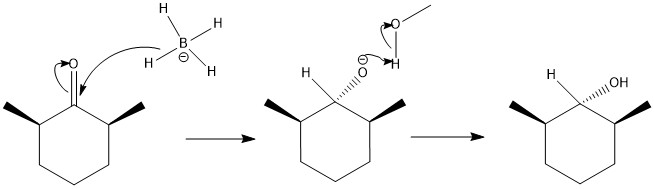
\includegraphics[height = 3.5cm, width = 12cm]{mikroskaalmekanismi.jpg}

\vspace{0.3cm}

\section{Työn suoritus}

\noindent Pieneen koeputkeen laimennettiin kaupallista ketonia ($2 \mu$l) metanoliin ($250 \mu$l). Tämän jälkeen liuokseen lisättiin spaatelikärjen verran kiinteätä natriumboorihybridiä (NaBH$_4$). Koeputkea ravistettiin sen verran, että NaBH$_4$ liukeni kokonaan liuokseen. Annettiin NaBH$_4$ reagoida ketonin kanssa keskenään 10 minuuttia. 

Annettuaan ketonin pelkistyä, lisättiin NaCO$_3$ (0,5ml) ja heksaania (2ml). Tätä liuosta ravistettiin ja annettiin istua pariksi minuutiksi, että näkyvä faasi erottui. Pelkistynyttä ketonia , 2,6-dimetyylisykloheksanoni, otettiin 1ml verran, joka on ylemmässä kerroksessa. Näyte pistettiin käyttyn heksaanin ja kaupallisen ketonin kanssa GC:lle ajettavaksi. Kaasugromatogrammien avulla selvitettiin heksaanin puhtaus, ketoni isomeerien suhde ja pelkistettyjen tuotteiden suhde. 


\section{Johtopäätökset}

Liitteestä \textbf{Kromatogrammi: Kaupallinen ketoni}:sta nähdään, että käytetyssä kaupallisessa ketonissa löytyy sekä \textbf{1} ja \textbf{2} isomereita. Kromatogramissa ne esiintyy eri suuruisina piikkeinä. Taulukon mukaan 5-6 minuutin kohdalla esiintyy kaksi piikkiä joiden suhde $89:11 \approx 8:1$. 

Tässä vaiheessa ei vielä tiedätä mikä piikki on mikäkin isomeria. Tämän saatiin selville tutkimalla \textbf{Kromatogrammi: Tuotteet}. Kromatogrammissä nähdään kolme eri piikkiä, joista kaksi 5-6 minuutin kohdalla ovat vierekkäin ja yksi piikki kauempana 6,5 minuutin kohdalla. Kromatogrammista nähdään, että 5-6 minuutin olevat piikit ovat integraaliltaan suurin. Nämä piikit esittävät \textbf{Reaktioyhtälö}:n mukaan isomeereja \textbf{3} ja \textbf{4}, jossa pidempi piikki on \textbf{3} ja pienempi \textbf{4}. 6,5 minuutin kohdalla oleva piikki esittää isomeeriat \textbf{5} ja \textbf{6}.

Kromatogrammin mukaan tuotteista $25.43 \%$ oli isomeriaa \textbf{4}, $67.03\%$ \textbf{3}:a ja $7.54\%$ \textbf{5}:ttä ja \textbf{6}:tta. Eli siis tuotteista yhteensä 92.46$\%$ ovat isomeereja \textbf{3} ja \textbf{4}, mitkä ovat ketoni-isomerista \textbf{1} pelkistettyjä tuotteita.

Osana työn tehtävänä oli myös tarkastella käyttämämme liuottimen puhtautta. Liuottimena käytettiin heksaania ja sen puhtautta tarkattettiin sen kromatokrammin avulla. Liitteessä \textbf{Kromatogrammi: Heksaani}:ssa kuvataan heksaanin puhtautta. Sillä kromatogrammissa ei esiinny mitään muuta huomattavan suurta piikkiä, niin voidaan sanoa heksaanin olevan puhdasta. 

Näiden avulla voidaan sanoa, että käytyssä kaupallisessa ketonissa sisältää pääosin (89.23$\%$) \textit{cis}-2,6-dimetyyliheksanonia. Tuotteista \textit{trans,\- trans}-2,6-dimetyyliheksanolia esiintyy ylivoimaisesti eniten ja ketonin \textit{trans}-isomerian tuottama enantiomeerit \textit{cis,trans}-2,6-dimetyyliheksanolia esiintyy vain $7.54\%$.  Yksi selitys tuotteiden suhteista voi olla esimerkiksi reagenssin, NaBH$_4$, hyökkäys suunnasta. 

\noindent



\pagebreak


\section{Viiteet}

\noindent 1. Garner, C.M., \textit{Journal of Chemical education}, \textbf{1993}, 70, A310.

\section{Liiteet}

\noindent Kromatogrammi: Heksaani

\noindent Kromatogrammi: Kaupallinen ketoni

\noindent Kromatogrammi: Tuotteet

\end{document}
